\section{Sesión 7}

\begin{lema}
	Sean $f,g \in R[a,b]$. Para cada $P\in P[a,b]$ y cualquier selección de números $t_1,t_2,\cdots, t_n$, donde $t_k\in [x_{k-1},x_k]$, y cualquier selección de números $f_1,f_2,\cdots, f_n$, con $f_k\in \{M_k(f), m_k(f)\}$, considere 
	$$w(P,f,g)=\sum_{k=1}^n f_k g(t_k)\Delta x_k.$$
\end{lema}

\begin{teorema}(Bonnet)
	Sean $f\in R[a,b]$ y $g$ una función no negativa, acotada y monótona decreciente. Entonces, $\exists \mu \in [a,b]\ni$ 
	$$\int_a^b fg=g(a)\int_a^\mu f.$$
\end{teorema}

\begin{teorema}
	Suponga que $f,g\in C[a,b]$ y $f$ y $g$, son difereciables en $(a,b)$. Suponga, además, que $f'$, $g'\in R[a,b]$. Entonces, 
	$$\int_a^b fg'dx=f(b)g(b)-f(a)g(a)-\int_a^b f'g dx.$$
\end{teorema}

\begin{teorema}
	Suponga que $g:I\to\mathbb{R}$ es diferenciable y que $g'$ es integrable en $I$. Sea $g(I)=J$. Si $f:J\to\mathbb{R}$, entonces, $\forall a, b\in I$, se cumple: 
	
	$$\int_a^b f(g(x))\cdot g'(x)dx=\int_{g(a)}^{g(b)}f(u)du.$$
\end{teorema}
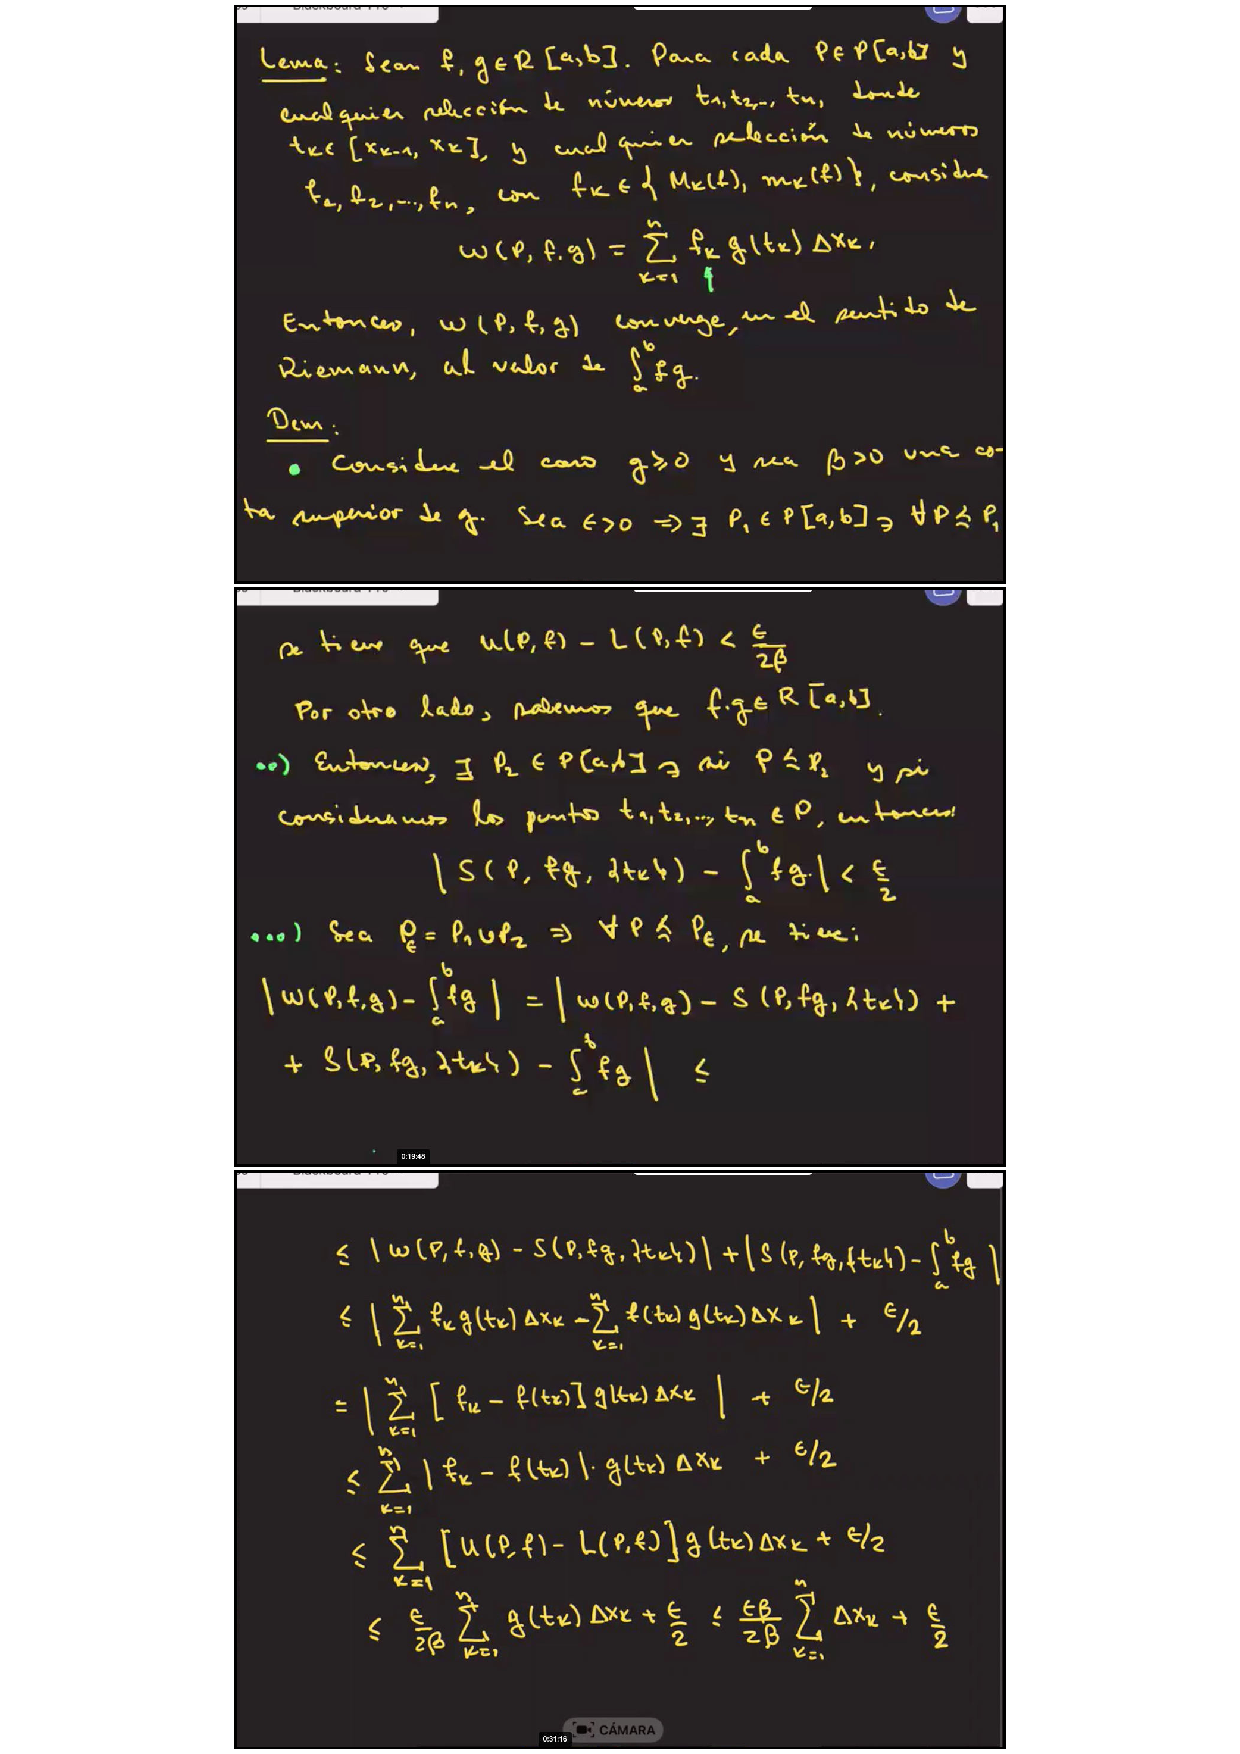
\includepdf[pages=-]{apendices/s7.pdf}